In this section the main architectural decision are explained to better specify how a specific decision may affect 
the system to be.
\subsubsection{Multitier architecture}
The client-server architecture is implemented using a multitier architecture. In this way the Business Logic, the presentation and the Data Storage tier are maintained separated and isolated. Therefore, the application remains flexible and every tier can be implemented, tested and modified separately from the others.\\
In particular:

\begin{itemize}
    \item \textit{Presentation tier:} this is the only part of the system-to-be accessible directly from the user. Its purpose is to translate action of the user into action and requests to the System and translate back the response of the System into something human readable.
    
    
    \item \textit{Web tier:} the purpose of this layer is to provide to the Company Web browser the web pages. The server does not have a connection with the Business Logic tier because it hasn't the need to make requests directly. Indeed, the web application will make the necessary requests directly to the Business Logic tier, modifying the webpage directly.
    
    \item \textit{Business Logic tier:} this is the central tier as it contains the logic of the application. It is responsible of processing the user requests and saving data into the database. In the architecture proposed, this tier contains also the reverse proxy, a component that is needed in order to balance the user-generated network traffic to the multiple servers.
    
    \item \textit{Data storage tier:} this component is actually a database; its purpose is to maintain the state of the data and ensure it persistence.
\end{itemize}
\begin{figure}[H]
	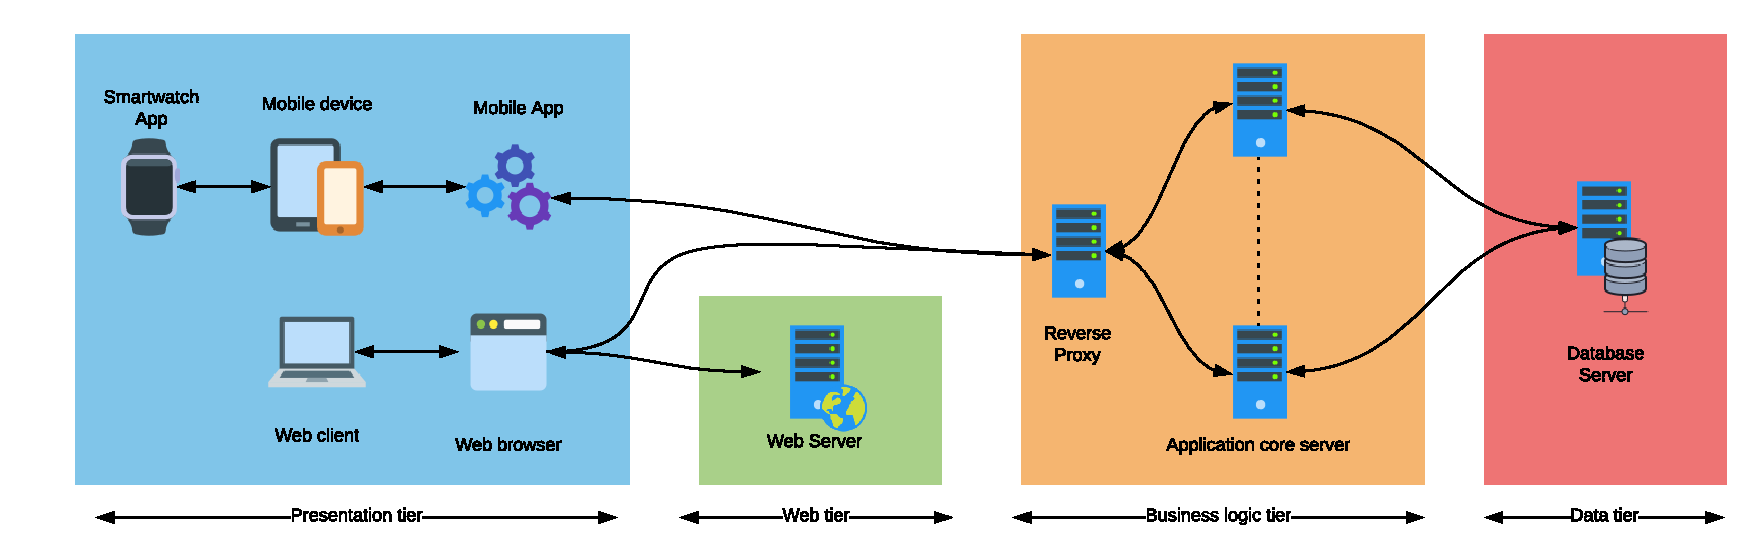
\includegraphics[width=\textwidth,height=\textheight,keepaspectratio]{assets/MultiTierSystem.pdf}
	\caption{Multitier view of the system}
	\label{fig:MultiTierSystem}
\end{figure}

\subsubsection{Thin client}
The system will use a Thin client paradigm that will handle only communications with the main server.
Using a Fat client paradigm is not convenient in this case because our customers rely mostly on Mobile phones which can have troubles in handle computational effort.
The server of Data4Help will have sufficient computational power to manage a lot of user requests at the same time.

\subsubsection{RESTful}
The communication between the Core and the smartwatch App / Web site is made using a RESTful (Representational State Transfer) service, that means that all the query are simple HTTP query, so a security layer can be easily added using SSL/HTTPS. Moreover, the RESTful was formalized with scalability in mind, so that a web service implemented using a RESTful architecture can be easily expanded to fulfill new needs.
Being a simple HTTP request, it is compatible with all firewall/proxy, simplifying the configuration aspects of the system, and as the response body JSON can be used, a fully standardized and powerful but simple language to exchange data.
